\subsection{Results distribution}
\begin{center}  
\begin{minipage}{.55\textwidth}
\begin{center}
\includegraphics[width=\textwidth,keepaspectratio]{{../Results/50Trials/Distributions}.pdf}

\vskip15pt
(a)
\vskip15pt


\end{center}
\end{minipage}%
\hspace{0.5cm}
\begin{minipage}{.35\textwidth}
\begin{footnotesize}
\begin{center}

\begin{tabular}{|l|c|c|}
\hline
& \multicolumn{1}{p{2cm}|}{\textbf{Robots in Chain}} & \multicolumn{1}{p{2cm}|}{\textbf{Completion Time}} \\
\hline
\textbf{Mean} &	36.82 & 21779.52 \\
\hline
\textbf{Std Dev} & 2.5689671 & 11138.0954867 \\
\hline
 \textbf{CV} = $\frac{\sigma}{\mu}$ & 0.06952743 &	0.51140223 \\
\hline
 \textbf{Median} & 37 &	21209.5 \\
\hline
\textbf{Min} & 30 & 6133 \\
\hline
\textbf{Max} & 41 & 47097 \\
\hline
\end{tabular}
\label{tab:summary}

\vskip15pt
(b)
\vskip15pt


\end{center}
\end{footnotesize}
\end{minipage}
\captionof{figure}{Panel containing the histograms and the empirical cumulative distribution functions for the designed metrics (a) with a summary of the relevant statistics of the two distributions (b)}
\end{center}

The analysis of the distribution of these metrics shows that, in the 90\% of the experiments, the number of robots required to form a chain is bounded in the interval $[32,40]$.

The variability of this results can be explained by the nature of the targets and their placement in the environment.
In fact, since the spots can only be sensed if a robot is completely on it, sometimes it may happen that a robot ignores the presence of the spot, even while being next to it, and tries to extend the chain in another direction, with respect to the target.

On the other hand, even though approximately the 75\% of the trials are completed within 30000 simulation steps, there is a great variability in the time required to successfully complete the task, as shown by the variation coefficient (CV).

Given the nature of the method, the change in the value of the seed will affect only the initial deployment position and rotation and the stopping position of the first robot (cf. \nameref{sec:sm}).

One can then conclude that the random change in the seed has a relevant impact on the completion time, while having a minor influence on the number of robots in the chain, that can be partially explained by the nature of the environment.

\subsection{Scatterplot and correlation analysis}

\begin{center}  
\begin{minipage}{.55\textwidth}
\begin{center}
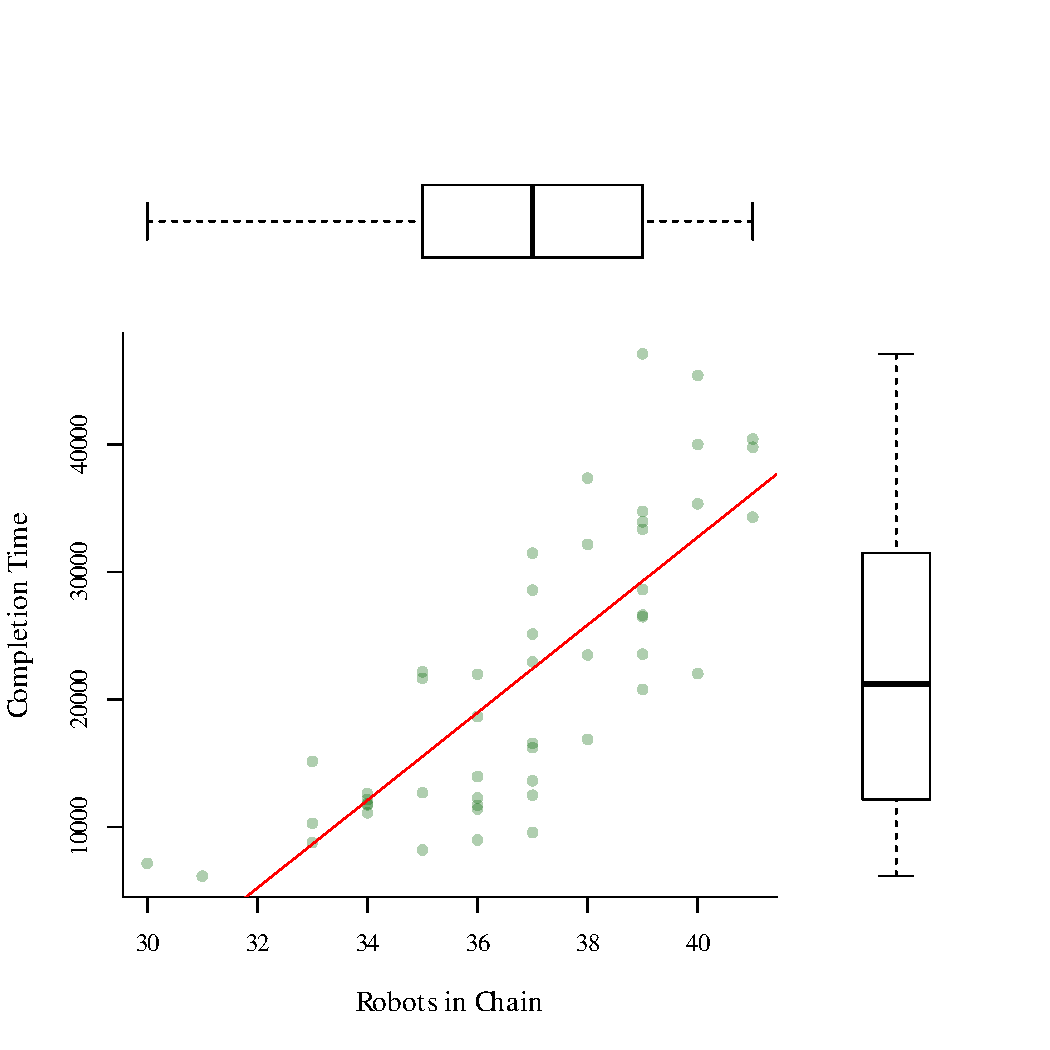
\includegraphics[width=\textwidth,keepaspectratio]{{../Results/50Trials/ResultsDistribution}.pdf}

(a)

\end{center}
\end{minipage}%
\hspace{0.5cm}
\begin{minipage}{.35\textwidth}
\begin{footnotesize}
\begin{center}

\begin{tabular}{|l|c|c|}
\hline
& \textbf{Value} & \textbf{P-Value} \\
\hline
\textbf{Pearson - } $\mathbf{r}$  &	0.7934599 & 6.357e-12 \\
\hline
\textbf{Kendall -} $\mathbf{\tau}$ & 0.6691023 & 5.554e-11 \\
\hline
\end{tabular}
\label{tab:correlation}
\vskip15pt
(b)
\vskip15pt

\end{center}
\end{footnotesize}
\end{minipage}
\captionof{figure}{Enhanced scatter plot of the completion times as a function of the number of robots (a), with the results of the correlation analysis (b)}
\end{center}

Intuitively, one may assume that the completion time is positively correlated with respect to the number of robots in chain (since more robots require more time to be deployed).

This intuition is confirmed by the graphical representation of the completion time as a function of the number of robots in the chain, along with the representation of a linear model fitting the points obtained through the experiment as well as by the values of the correlation coefficients, and their statistical significance (attested by a p-value considerably small than the confidence level $1-\alpha=0.05$.

\bibliographystyle{plain}
\bibliography{References}
